\subsection{A Negative Coordinate Means Motion in the Opposite Direction}

\begin{examplebox}
The example $[\mathbf u]_{\mathcal B}=(2,1)$ used positive coefficients. That
is convenient for drawing a parallelogram, but basis coordinates need not be
positive.

Keep
\[
\mathbf b_1=(2,1),
\qquad
\mathbf b_2=(1,2),
\]
and consider
\[
\mathbf w=2\mathbf b_1-\mathbf b_2.
\]
Calculating with ordinary coordinate pairs gives
\[
\mathbf w
=2(2,1)-(1,2)
=(4,2)-(1,2)
=(3,0).
\]
Therefore
\[
[\mathbf w]_{\mathcal E}=(3,0),
\qquad
[\mathbf w]_{\mathcal B}=(2,-1).
\]

\begin{center}
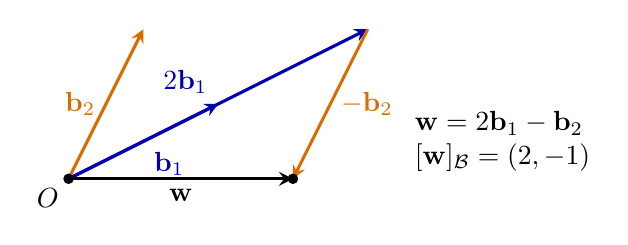
\begin{tikzpicture}[scale=0.95,>=stealth]
    \coordinate (O) at (0,0);
    \coordinate (B1) at (2,1);
    \coordinate (B2) at (1,2);
    \coordinate (TwoB1) at (4,2);
    \coordinate (W) at (3,0);

    \draw[blue!70!black,line width=1.1pt,->] (O) -- (B1)
        node[midway,below right] {$\mathbf b_1$};
    \draw[orange!85!black,line width=1.1pt,->] (O) -- (B2)
        node[midway,left] {$\mathbf b_2$};
    \draw[blue!70!black,line width=1.1pt,->] (O) -- (TwoB1)
        node[midway,above left] {$2\mathbf b_1$};
    \draw[orange!85!black,line width=1.1pt,->] (TwoB1) -- (W)
        node[midway,right] {$-\mathbf b_2$};
    \draw[very thick,->] (O) -- (W)
        node[midway,below] {$\mathbf w$};

    \fill (O) circle (2pt) node[below left] {$O$};
    \fill (W) circle (2pt);
    \node[align=left,anchor=west] at (4.5,0.5)
        {$\mathbf w=2\mathbf b_1-\mathbf b_2$\\
         $[\mathbf w]_{\mathcal B}=(2,-1)$};
\end{tikzpicture}
\end{center}

The coefficient $-1$ does not mean a negative length. It means one copy of
$\mathbf b_2$ taken in the opposite direction. Basis coordinates are signed
instructions for reconstructing the vector.
\end{examplebox}
